\chapter{METODOLOGI DAN RANCANGAN PENELITIAN}

\section{Metodologi Penelitian}
Penelitian ini menerapkan metode \textit{Prototyping} untuk memungkinkan pengembangan sistem secara bertahap dan iteratif. Pendekatan ini dipilih karena sesuai dengan karakteristik sistem \textit{Reinforcement Learning} yang memerlukan proses evaluasi dan perbaikan secara berulang untuk mencapai performa yang optimal.

Metode Prototyping dalam penelitian ini dilakukan melalui beberapa tahapan utama, yaitu identifikasi kebutuhan sistem, perancangan sistem awal, pembangunan prototipe, pengujian sistem, serta evaluasi dan perbaikan. Setiap tahap dilakukan secara berulang hingga sistem yang dikembangkan mampu mencapai tujuan yang diharapkan.

\begin{figure}[H]
\centering
\resizebox{0.95\textwidth}{!}{
\begin{tikzpicture}[
    node distance=0.65cm and 0.8cm,
    auto,
    process/.style={
        draw, rectangle, rounded corners, 
        minimum width=5.5cm, minimum height=0.75cm, 
        align=center, fill=blue!10, font=\scriptsize\sffamily
    },
    process_split/.style={
        draw, rectangle, rounded corners, 
        minimum width=4.5cm, minimum height=0.75cm, 
        align=center, fill=blue!10, font=\scriptsize\sffamily
    },
    decision/.style={
        draw, diamond, aspect=2,
        minimum width=3.3cm, minimum height=0.85cm, 
        align=center, fill=green!10, font=\scriptsize\sffamily
    },
    startstop/.style={
        draw, rectangle, rounded corners, 
        minimum width=3.8cm, minimum height=0.85cm, 
        align=center, fill=red!10, font=\scriptsize\sffamily
    },
    arrow/.style={
        -Stealth, thick
    }
]

    % Alur Utama Atas (Gunakan koordinat atau placeholder jika bagian atas ingin dipastikan presisi)
    \node (n1) [process] {Studi Literatur};
    \node (n2) [process, below=of n1] {Identifikasi Kebutuhan Sistem};
    \node (n3) [process, below=of n2] {Perancangan Sistem Awal};
    \node (n4) [process, below=of n3] {Perancangan Komponen \textit{Q-Learning}\\
    \textit{State, Action, Reward, Q-Table, Hyperparameter}};
    \node (n5) [process, below=of n4] {Pembangunan Prototipe Sistem};

    % Alur Paralel (Bercabang ke Kiri dan Kanan)
    \node (n6) [process_split, below left=0.8cm and -1.8cm of n5] {Pengujian \textit{Baseline}\\Menggunakan OWASP ZAP};
    \node (n7) [process_split, below right=0.8cm and -1.8cm of n5] {Pengujian Sistem Berbasis\\\textit{Reinforcement Learning}};

    % Alur Penggabungan Bawah
    \node (n8) [process, below=2.3cm of n5] {Evaluasi dan Analisis Hasil};
    \node (n9) [decision, below=of n8] {Sesuai\\Tujuan?};
    \node (n10) [startstop, right=of n9, xshift=1.2cm] {Produk Akhir};

    % Menghubungkan Garis Panah
    \draw [arrow] (n1) -- (n2);
    \draw [arrow] (n2) -- (n3);
    \draw [arrow] (n3) -- (n4);
    \draw [arrow] (n4) -- (n5);
    
    % Panah dari Prototipe ke Cabang Pengujian
    \draw [arrow] (n5.south) -- (n6.north);
    \draw [arrow] (n5.south) -- (n7.north);
    
    % Panah dari Pengujian ke Evaluasi
    \draw [arrow] (n6.south) -- (n8.north);
    \draw [arrow] (n7.south) -- (n8.north);
    
    \draw [arrow] (n8) -- (n9);
    \draw [arrow] (n9) -- node [anchor=south, font=\scriptsize] {Ya} (n10);

   
    \draw [arrow] (n9.west) -- ++(-4.8,0) |- (n3.west) 
        node [pos=0.85, above, font=\scriptsize, xshift=0.3cm] {Tidak / Perbaikan};

\end{tikzpicture}
}
\caption{Alur Metodologi Penelitian}
\label{fig:alur_metodologi_penelitian}
\end{figure}

\section{Alat dan Bahan yang Digunakan}

\subsection{Perangkat Lunak}

\begin{table}[H]
\centering
\begin{tabular}{|c|l|p{8cm}|}
\hline
\textbf{No} & \textbf{Komponen} & \textbf{Keterangan} \\ \hline

1 & Bahasa Pemrograman & Python dengan library NumPy untuk perhitungan Q-Table dan Requests untuk komunikasi HTTP \\ \hline

2 & Metode RL & Q-Learning sebagai algoritma pembelajaran agen \\ \hline

3 & Target Lingkungan & OWASP Juice Shop \\ \hline

4 & Tools Pendukung & OWASP ZAP digunakan sebagai baseline pengujian dan integrasi melalui API \\ \hline

5 & Editor Kode & Visual Studio Code \\ \hline

\end{tabular}
\caption{Perangkat Lunak yang Digunakan}
\end{table}

\subsection{Perangkat Keras}

\begin{table}[H]
\centering
\begin{tabular}{|c|l|p{8cm}|}
\hline
\textbf{No} & \textbf{Komponen} & \textbf{Spesifikasi} \\ \hline

1 & Laptop/PC & Perangkat utama yang digunakan untuk menjalankan proses pengembangan sistem, pengujian, dan analisis hasil \\ \hline

2 & RAM & Minimal 8 GB \\ \hline

3 & Prosesor & Minimal Intel i5 atau setara \\ \hline

\end{tabular}
\caption{Perangkat Keras yang Digunakan}
\end{table}

\section{Perancangan Sistem Awal / Arsitektur Solusi}

\subsection{Analisis Aktor}

Analisis aktor dilakukan untuk mengidentifikasi komponen-komponen yang terlibat dalam sistem \textit{automated penetration testing} berbasis \textit{Reinforcement Learning}. Setiap aktor memiliki peran dan tanggung jawab masing-masing dalam mendukung proses pengujian keamanan secara otomatis dan adaptif. Pada penelitian ini, terdapat tiga aktor utama, yaitu Administrator, \textit{RL Agent}, dan \textit{Environment} berupa aplikasi \textit{OWASP Juice Shop}.

Administrator berperan sebagai pihak yang melakukan konfigurasi awal sistem sebelum proses pengujian dijalankan. Tugas administrator meliputi penentuan parameter pelatihan seperti \textit{learning rate}, nilai \textit{epsilon}, jumlah episode, serta pengaturan skenario pengujian yang akan digunakan. Selain itu, administrator juga bertanggung jawab dalam memantau hasil pengujian, mengevaluasi performa agen, serta menganalisis kerentanan yang berhasil ditemukan selama proses \textit{penetration testing}. Peran administrator sangat penting untuk memastikan sistem berjalan sesuai tujuan penelitian.

\textit{RL Agent} merupakan komponen inti dalam sistem yang berfungsi sebagai agen pembelajar. Agen bertugas menentukan aksi atau strategi pengujian yang akan dilakukan berdasarkan kondisi lingkungan yang diamati. Dalam prosesnya, agen akan menerima informasi berupa \textit{state} dari lingkungan, kemudian memilih tindakan tertentu seperti mengirimkan \textit{payload}, melakukan eksplorasi endpoint, atau mencoba pola serangan tertentu. Setelah aksi dilakukan, agen akan menerima \textit{reward} sebagai umpan balik atas keberhasilan atau kegagalan tindakan tersebut. Melalui mekanisme ini, agen dapat mempelajari strategi pengujian yang paling optimal secara bertahap.

Sementara itu, \textit{environment} dalam penelitian ini direpresentasikan oleh aplikasi \textit{OWASP Juice Shop} yang berfungsi sebagai target pengujian keamanan. Aplikasi ini dipilih karena memiliki berbagai jenis kerentanan keamanan web yang sesuai untuk kebutuhan simulasi \textit{penetration testing}. \textit{Environment} akan memberikan respons terhadap setiap aksi yang dilakukan oleh agen, seperti respons HTTP, status keberhasilan eksploitasi, maupun perubahan kondisi sistem tertentu. Respons tersebut kemudian digunakan sebagai dasar bagi agen untuk menentukan langkah pengujian berikutnya.

Interaksi antara administrator, \textit{RL Agent}, dan \textit{environment} membentuk suatu siklus pembelajaran yang berkelanjutan. Administrator melakukan konfigurasi sistem, agen menjalankan proses pengujian dan pembelajaran, sedangkan \textit{environment} menyediakan umpan balik yang digunakan agen untuk meningkatkan performanya. Dengan adanya interaksi tersebut, sistem diharapkan mampu melakukan \textit{automated penetration testing} secara lebih adaptif dibandingkan pendekatan konvensional berbasis aturan.

\usetikzlibrary{positioning, fit, arrows.meta, backgrounds}

\subsection{Keterkaitan Rancangan Sistem dengan Permasalahan Penelitian}

Rancangan sistem dalam penelitian ini disusun untuk menjawab permasalahan utama yang telah dijelaskan pada Bab 1, yaitu keterbatasan metode \textit{automated web penetration testing} konvensional dalam aspek adaptivitas dan efisiensi. Pada metode konvensional, proses pengujian umumnya dilakukan berdasarkan aturan atau daftar \textit{payload} yang telah ditentukan sebelumnya. Pendekatan tersebut cenderung menjalankan banyak percobaan tanpa mempertimbangkan hasil dari pengujian sebelumnya, sehingga dapat menghasilkan jumlah \textit{request} yang besar dan proses pengujian yang kurang efisien.

Untuk menjawab permasalahan tersebut, sistem yang dirancang dalam penelitian ini menggunakan pendekatan \textit{Reinforcement Learning} dengan algoritma Q-Learning. Agen tidak hanya mengirimkan \textit{payload} secara berulang, tetapi juga mempelajari hasil dari setiap aksi berdasarkan respons aplikasi target. Respons tersebut digunakan untuk membentuk \textit{state} dan memberikan nilai \textit{reward}, sehingga agen dapat memperbarui Q-Table dan menentukan strategi pengujian yang lebih tepat pada iterasi berikutnya.

Dengan rancangan tersebut, aspek adaptivitas dijawab melalui kemampuan agen dalam memilih aksi berdasarkan pengalaman sebelumnya, sedangkan aspek efisiensi dijawab melalui pengukuran jumlah \textit{request}, waktu pengujian, dan tingkat keberhasilan identifikasi kerentanan. Oleh karena itu, rancangan sistem tidak hanya menjelaskan implementasi metode, tetapi juga menunjukkan bagaimana metode yang diusulkan digunakan untuk menjawab problem utama penelitian.

\subsection{Arsitektur Sistem}
Sistem yang dikembangkan dirancang agar agen \textit{Reinforcement Learning} dapat melakukan proses \textit{penetration testing} melalui alur yang terintegrasi dari pengumpulan informasi hingga pemindaian kerentanan. Arsitektur sistem ditunjukkan pada Gambar \ref{fig:arsitektur_baru}.

\begin{figure}[h!]
\centering
\resizebox{\textwidth}{!}{
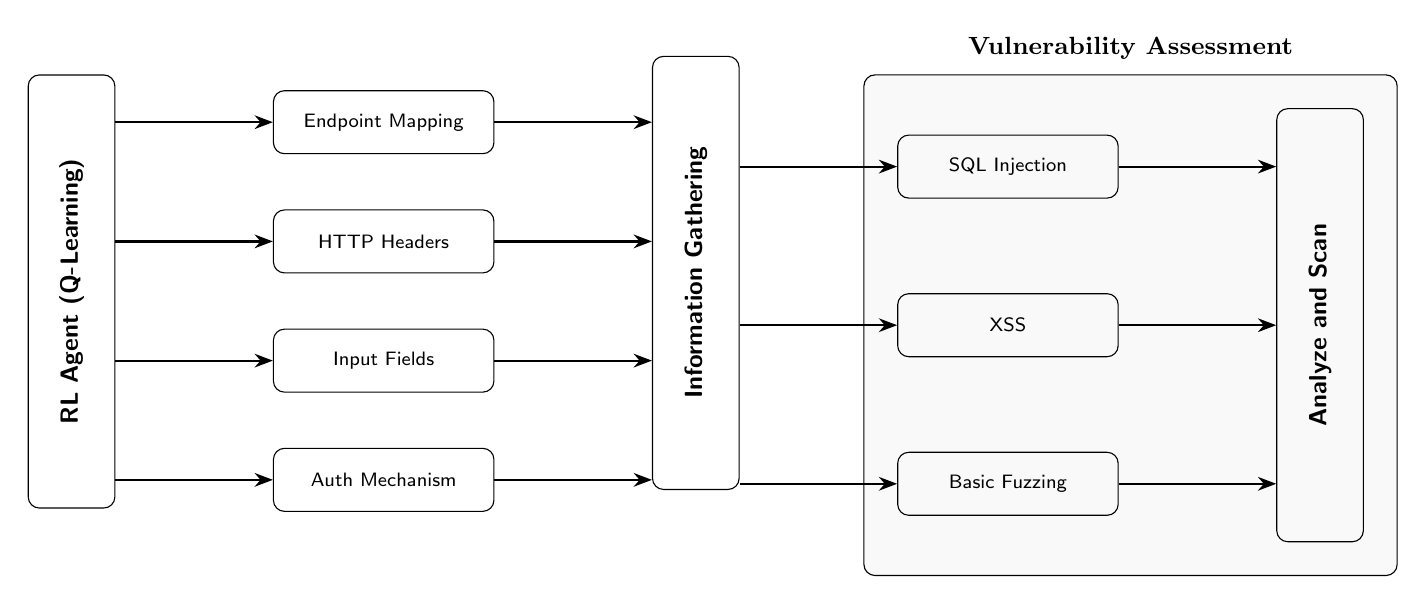
\begin{tikzpicture}[
    node distance=0.7cm and 1.2cm,
    block/.style={draw, rectangle, rounded corners, minimum width=2.8cm, minimum height=0.8cm, text centered, font=\scriptsize\sffamily},
    tallblock/.style={draw, rectangle, rounded corners, minimum width=1.1cm, minimum height=5.5cm, text centered, font=\small\bfseries\sffamily},
    arrow/.style={-Stealth, thick}
]

    \node (agent) [tallblock] {\rotatebox{90}{RL Agent (Q-Learning)}};

    \node (f1) [block, right=of agent.north east, anchor=north west, xshift=0.8cm, yshift=-0.2cm] {Endpoint Mapping};
    \node (f2) [block, below=of f1] {HTTP Headers};
    \node (f3) [block, below=of f2] {Input Fields};
    \node (f4) [block, below=of f3] {Auth Mechanism};

    \node (info) [tallblock, right=of f2, xshift=0.8cm, yshift=-0.4cm] {\rotatebox{90}{Information Gathering}};

    \node (v1) [block, right=of info.north east, anchor=north west, xshift=0.8cm, yshift=-1cm] {SQL Injection};
    \node (v2) [block, below=of v1, yshift=-0.5cm] {XSS};
    \node (v3) [block, below=of v2, yshift=-0.5cm] {Basic Fuzzing};

    \node (scan) [tallblock, right=of v2, xshift=0.8cm] {\rotatebox{90}{Analyze and Scan}};

    \begin{scope}[on background layer]
        \node[draw, rectangle, rounded corners, fill=gray!5, inner sep=12pt, fit=(v1) (v3) (scan), label={[font=\small\bfseries, yshift=2pt]above:Vulnerability Assessment}] (va_box) {};
    \end{scope}

    \foreach \n in {f1, f2, f3, f4} {
        \draw [arrow] (agent.east |- \n.west) -- (\n.west);
    }

    \foreach \n in {f1, f2, f3, f4} {
        \draw [arrow] (\n.east) -- (info.west |- \n.east);
    }

    \foreach \n in {v1, v2, v3} {
        \draw [arrow] (info.east |- \n.west) -- (\n.west);
    }

    \foreach \n in {v1, v2, v3} {
        \draw [arrow] (\n.east) -- (scan.west |- \n.east);
    }

\end{tikzpicture}
}
\caption{Arsitektur Sistem Penetration Testing Berbasis Reinforcement Learning}
\label{fig:arsitektur_baru}
\end{figure}

Berdasarkan Gambar \ref{fig:arsitektur_baru}, proses dimulai dari \textit{RL Agent} yang menentukan aksi berupa strategi pengujian. Aksi tersebut dikirimkan ke \textit{Pentest Engine} untuk menghasilkan \textit{HTTP request} yang akan dikirimkan ke aplikasi target \textit{OWASP Juice Shop}. Respons yang diterima kemudian dianalisis oleh \textit{Response Analyzer} untuk menghasilkan \textit{state} baru serta \textit{reward}, yang selanjutnya digunakan untuk memperbarui strategi agen.

Untuk memberikan gambaran yang lebih implementatif, arsitektur sistem dikembangkan menjadi lebih rinci seperti ditunjukkan pada Gambar \ref{fig:arsitektur_detail}.

\begin{figure}[h!]
\centering
\resizebox{\textwidth}{!}{
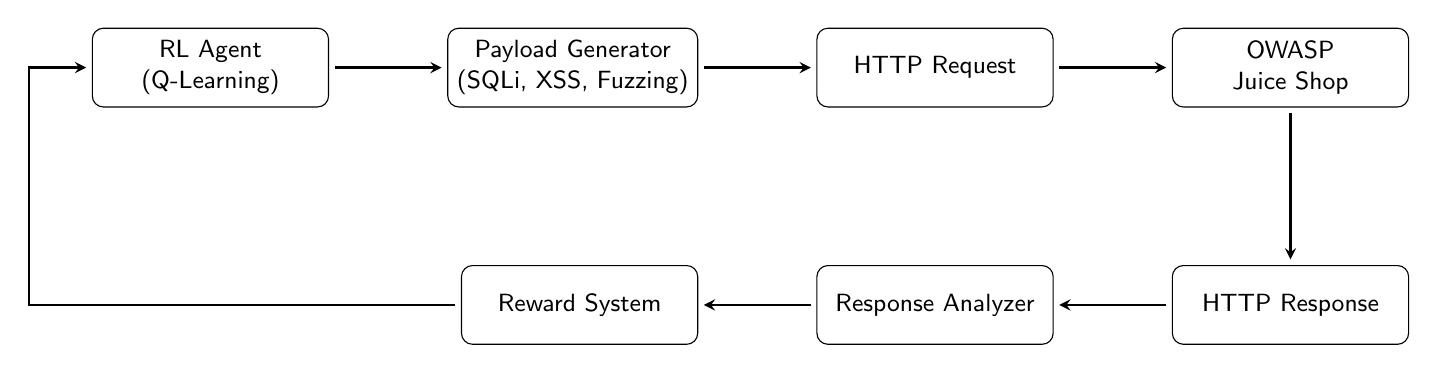
\begin{tikzpicture}[
    node distance=1.2cm and 1.5cm,
    block/.style={
        draw, 
        rectangle, 
        rounded corners=4pt, 
        minimum width=3cm, 
        minimum height=1cm, 
        align=center,
        fill=white,
        font=\small\sffamily
    },
    arrow/.style={
        ->, 
        >=stealth,
        thick, 
        shorten >=2pt, 
        shorten <=2pt
    }
]

\node[block] (agent) {RL Agent\\(Q-Learning)};
\node[block, right=of agent] (payload) {Payload Generator\\(SQLi, XSS, Fuzzing)};
\node[block, right=of payload] (request) {HTTP Request};
\node[block, right=of request] (target) {OWASP\\Juice Shop};

\node[block, below=2cm of target] (response) {HTTP Response};
\node[block, left=of response] (analyzer) {Response Analyzer};
\node[block, left=of analyzer] (reward) {Reward System};

\draw[arrow] (agent) -- (payload);
\draw[arrow] (payload) -- (request);
\draw[arrow] (request) -- (target);
\draw[arrow] (target) -- (response);
\draw[arrow] (response) -- (analyzer);
\draw[arrow] (analyzer) -- (reward);

\draw[arrow] (reward.west) -| ([xshift=-0.8cm]agent.west) -- (agent.west);

\end{tikzpicture}
}
\caption{Arsitektur Sistem Secara Detail}
\label{fig:arsitektur_detail}
\end{figure}

Pada Gambar \ref{fig:arsitektur_detail}, proses pengujian ditunjukkan secara lebih rinci. Agen \textit{Reinforcement Learning} memilih aksi berupa \textit{payload} tertentu, seperti \textit{SQL Injection}, \textit{Cross-Site Scripting} (XSS), atau \textit{fuzzing}. Payload tersebut dikirimkan melalui modul \textit{HTTP Request} menggunakan library Python ke aplikasi target. Respons yang diterima dianalisis untuk mengidentifikasi indikasi kerentanan, kemudian digunakan untuk menentukan nilai \textit{reward}. Nilai ini selanjutnya digunakan untuk memperbarui \textit{Q-Table}, sehingga agen dapat meningkatkan strategi pengujian secara adaptif pada iterasi berikutnya.

\subsection{Desain Komponen Reinforcement Learning}

Model \textit{Reinforcement Learning} dalam penelitian ini terdiri dari tiga komponen utama, yaitu \textit{state}, \textit{action}, dan \textit{reward}. \textit{State} (S) direpresentasikan sebagai kombinasi fitur dari respons sistem, seperti \textit{status code}, panjang respons, dan indikator error, yang kemudian diolah dalam bentuk representasi diskrit, misalnya tuple, agar dapat digunakan sebagai indeks dalam Q-Table.

\textit{Action} (A) merupakan aksi yang dilakukan oleh agen berupa pengiriman \textit{payload} ke aplikasi target. Payload yang digunakan dalam penelitian ini mencakup \textit{SQL Injection}, \textit{Reflected Cross-Site Scripting} (Reflected XSS), dan \textit{fuzzing}. Jenis XSS yang digunakan secara khusus adalah \textit{Reflected XSS}, bukan XSS secara umum, karena jenis serangan ini memberikan umpan balik yang lebih cepat dan terukur terhadap aksi yang dilakukan oleh agen. Pada Reflected XSS, payload dikirimkan melalui parameter URL atau input form, kemudian sistem menganalisis apakah payload tersebut muncul kembali pada respons HTTP. Karakteristik ini sesuai dengan kebutuhan Q-Learning karena keberhasilan atau kegagalan aksi dapat dievaluasi secara langsung melalui respons dari aplikasi target.

Sementara itu, \textit{reward} (R) diberikan sebagai umpan balik dari lingkungan. Nilai positif (+50) diberikan jika sistem berhasil menemukan indikasi kerentanan, misalnya ketika payload SQL Injection menghasilkan respons error tertentu atau ketika payload Reflected XSS berhasil muncul kembali pada isi respons HTTP tanpa proses sanitasi yang memadai. Sebaliknya, nilai negatif (-1) diberikan untuk setiap \textit{request} yang tidak menghasilkan temuan kerentanan. Selain itu, untuk mendukung proses pembelajaran, Q-Table direpresentasikan dalam bentuk struktur data seperti \textit{dictionary} dengan pasangan kunci \textit{(state, action)} dan nilai berupa estimasi $Q(s,a)$. Penentuan \textit{reward} ini bertujuan untuk mendorong agen menemukan kerentanan secara efisien dengan jumlah \textit{request} yang minimal \cite{nguyen2023}.

Agar komponen \textit{state}, \textit{action}, \textit{reward}, dan Q-Table dapat diimplementasikan secara sistematis, penelitian ini merancang struktur data utama yang digunakan dalam proses pengujian dan pembelajaran agen.

\subsection{Struktur Data Sistem}

Struktur data dalam penelitian ini dirancang untuk mendukung proses kerja sistem \textit{automated penetration testing} berbasis \textit{Reinforcement Learning}. Struktur data digunakan untuk menyimpan informasi yang diperoleh dari proses \textit{information gathering}, daftar \textit{payload} yang digunakan, respons dari aplikasi target, nilai \textit{reward}, serta Q-Table sebagai dasar pembelajaran agen.

Dalam sistem yang dikembangkan, struktur data berperan penting untuk memastikan bahwa setiap data yang diproses oleh agen dapat direpresentasikan secara terukur dan konsisten. Data yang digunakan tidak hanya berkaitan dengan hasil pengujian, tetapi juga mencakup representasi kondisi lingkungan atau \textit{state}, aksi yang dipilih oleh agen atau \textit{action}, dan nilai umpan balik atau \textit{reward} yang digunakan untuk memperbarui Q-Table.

\begin{table}[H]
\centering
\begin{tabular}{|c|l|l|p{6.5cm}|}
\hline
\textbf{No} & \textbf{Nama Struktur Data} & \textbf{Tipe Data} & \textbf{Keterangan} \\ \hline

1 & Endpoint Data & List/Array & Menyimpan daftar endpoint hasil proses \textit{endpoint mapping} pada aplikasi OWASP Juice Shop. \\ \hline
2 & Header Data & Dictionary & Menyimpan informasi HTTP header yang digunakan dalam proses pengiriman request. \\ \hline
3 & Input Field Data & List/Dictionary & Menyimpan informasi parameter atau field input yang dapat diuji menggunakan payload. \\ \hline
4 & Authentication Data & Dictionary & Menyimpan informasi mekanisme autentikasi yang diperlukan dalam proses pengujian. \\ \hline
5 & Payload Data & Dictionary/List & Menyimpan daftar payload berdasarkan kategori serangan, seperti SQL Injection, Reflected XSS, dan basic fuzzing. \\ \hline
6 & State Data & Tuple & Merepresentasikan kondisi lingkungan berdasarkan respons HTTP, seperti status code, panjang respons, indikator error, dan indikator refleksi payload. \\ \hline
7 & Action Data & String/Integer & Merepresentasikan aksi yang dipilih oleh agen, yaitu jenis payload atau strategi pengujian yang dilakukan. \\ \hline
8 & Reward Data & Integer/Float & Menyimpan nilai umpan balik yang diberikan kepada agen berdasarkan hasil analisis respons. \\ \hline
9 & Q-Table & Dictionary & Menyimpan nilai Q untuk setiap pasangan state dan action sebagai dasar pengambilan keputusan agen. \\ \hline
10 & Testing Log & List/Dictionary & Menyimpan riwayat pengujian, seperti endpoint, payload, status code, reward, dan indikasi kerentanan. \\ \hline

\end{tabular}
\caption{Struktur Data Utama Sistem}
\label{tab:struktur_data_utama}
\end{table}

\subsubsection{3.3.5.1 Struktur Data Endpoint}

Struktur data endpoint dirancang dengan poin-poin karakteristik sebagai berikut:

\begin{enumerate}
    \item \textbf{Fungsi Utama:} Digunakan untuk menyimpan daftar URL atau jalur (\textit{path}) unik yang diperoleh dari proses \textit{endpoint mapping}.
    \item \textbf{Peran Agen:} Menjadi target pengujian spesifik yang akan dikombinasikan dengan \textit{payload} tertentu berdasarkan keputusan agen \textit{Reinforcement Learning}.
    \item \textbf{Representasi Data:} Diimplementasikan dalam bentuk struktur linier (\textit{List/Array}) agar memudahkan proses iterasi pengujian.
\end{enumerate}

Contoh struktur data endpoint adalah sebagai berikut:

\begin{verbatim}
endpoint_data = [
    "/login",
    "/search",
    "/rest/products/search",
    "/api/Feedbacks"
]
\end{verbatim}

Setiap endpoint akan diuji menggunakan payload tertentu sesuai dengan aksi yang dipilih oleh agen. Dengan adanya struktur data ini, proses pengujian dapat dilakukan secara lebih sistematis karena agen memiliki daftar target yang jelas.

\subsubsection{3.3.5.2 Struktur Data HTTP Header}

Struktur data HTTP header memuat informasi dengan rincian elemen sebagai berikut:

\begin{enumerate}
    \item \textbf{Fungsi Utama:} Menyimpan informasi metadata \textit{header} yang dibutuhkan dalam proses komunikasi dan jabat tangan HTTP antara sistem penguji dan aplikasi target.
    \item \textbf{Komponen Konteks:} Menentukan format data, tipe konten (\textit{Content-Type}), identitas agen (\textit{User-Agent}), hingga token otorisasi keamanan.
    \item \textbf{Sifat Fleksibilitas:} Menggunakan struktur \textit{Key-Value Pair (Dictionary)} untuk mempermudah penambahan atau modifikasi \textit{header} secara dinamis sesuai kebutuhan \textit{state}.
\end{enumerate}

Contoh struktur data HTTP header adalah sebagai berikut:

\begin{verbatim}
header_data = {
    "Content-Type": "application/json",
    "User-Agent": "RL-Pentest-Agent",
    "Authorization": "Bearer <token>"
}
\end{verbatim}

Struktur ini digunakan oleh modul \textit{HTTP Request} saat mengirimkan payload ke aplikasi OWASP Juice Shop. Jika pengujian tidak membutuhkan autentikasi, maka bagian Authorization dapat dikosongkan atau tidak digunakan.

\subsubsection{3.3.5.3 Struktur Data Input Field}

Struktur data input field dirancang untuk menangani titik masuk data dengan spesifikasi sebagai berikut:

\begin{enumerate}
    \item \textbf{Fungsi Utama:} Menyimpan informasi parameter, variabel, atau \textit{field} input kontekstual yang dapat menerima masukan atau injeksi dari pengguna luar.
    \item \textbf{Target Serangan:} Memetakan area krusial tempat \textit{payload} SQL Injection, Reflected XSS, maupun \textit{fuzzing} dikirimkan (baik lewat URL, form input, maupun body request).
    \item \textbf{Efisiensi Agen:} Mencegah agen melakukan pengiriman \textit{payload} secara acak (\textit{blind fuzzing}) dan mengarahkannya langsung pada parameter yang valid dan memiliki potensi kerentanan.
\end{enumerate}

Contoh struktur data input field adalah sebagai berikut:

\begin{verbatim}
input_fields = [
    {
        "endpoint": "/login",
        "method": "POST",
        "parameters": ["email", "password"]
    },
    {
        "endpoint": "/search",
        "method": "GET",
        "parameters": ["q"]
    }
]
\end{verbatim}

Melalui struktur data ini, sistem dapat mengetahui parameter mana yang akan diuji menggunakan payload. Hal ini membantu agen agar pengiriman payload tidak dilakukan secara acak, melainkan diarahkan pada bagian aplikasi yang memiliki potensi menerima input.

\subsubsection{3.3.5.4 Struktur Data Authentication}

Struktur data authentication mengelola kredensial pengujian dengan poin-poin berikut:

\begin{enumerate}
    \item \textbf{Fungsi Utama:} Menyimpan informasi penanganan sesi, status \textit{state}, dan mekanisme pemeliharaan login pada sistem target.
    \item \textbf{Cakupan Skenario:} Memungkinkan pemindaian otomatis menembus \textit{endpoint} privat yang berada di balik dinding autentikasi (\textit{authenticated state}).
    \item \textbf{Atribut Kontrol:} Menyimpan status kebutuhan login (\textit{boolean flag}), tipe token (\textit{auth\_type}), dan nilai token aktif (\textit{session token}).
\end{enumerate}

Contoh struktur data authentication adalah sebagai berikut:

\begin{verbatim}
auth_data = {
    "is_required": True,
    "auth_type": "Bearer Token",
    "token": "<session_token>"
}
\end{verbatim}

Data autentikasi ini digunakan ketika agen perlu mengakses endpoint yang berada di balik mekanisme login. Dengan demikian, sistem dapat menjalankan pengujian pada endpoint publik maupun endpoint yang memerlukan autentikasi.

\subsubsection{3.3.5.5 Struktur Data Payload}

Struktur data payload mengorganisasi repositori serangan dengan pemetaan sebagai berikut:

\begin{enumerate}
    \item \textbf{Fungsi Utama:} Menyimpan string masukan eksploitasi (\textit{malicious vector}) yang digunakan oleh agen untuk menguji ketahanan sanitasi aplikasi target.
    \item \textbf{Kategorisasi Eksploitasi:} Mengelompokkan \textit{payload} secara terstruktur berdasarkan jenis kerentanan spesifik (SQL Injection, Reflected XSS, dan basic fuzzing).
    \item \textbf{Integrasi Modul:} Menjadi basis referensi utama bagi komponen \textit{Payload Generator} untuk menyuplai string serangan sesuai dengan \textit{action} yang dipilih agen.
\end{enumerate}

Contoh struktur data payload adalah sebagai berikut:

\begin{verbatim}
payload_data = {
    "sql_injection": [
        "' OR '1'='1",
        "' OR 1=1--",
        "admin'--"
    ],
    "reflected_xss": [
        "<script>alert(1)</script>",
        "<img src=x onerror=alert(1)>"
    ],
    "basic_fuzzing": [
        "../../../etc/passwd",
        "%00",
        "{{7*7}}"
    ]
}
\end{verbatim}

Struktur data payload berbentuk \textit{dictionary}, di mana setiap kategori serangan menjadi kunci utama dan daftar payload menjadi nilai dari kunci tersebut. Struktur ini memudahkan \textit{Payload Generator} dalam memilih payload sesuai aksi yang ditentukan oleh agen.

\subsubsection{3.3.5.6 Struktur Data State}

Struktur data state merepresentasikan umpan balik lingkungan dengan karakteristik sebagai berikut:

\begin{enumerate}
    \item \textbf{Fungsi Utama:} Menjadi representasi matematis dari kondisi lingkungan (\textit{environment state}) setelah suatu aksi pengujian (\textit{action}) dieksekusi.
    \item \textbf{Struktur Imutabilitas:} Menggunakan tipe data \textit{Tuple} untuk memastikan nilai status tidak berubah selama proses pencarian indeks pada Q-Table.
    \item \textbf{Dimensi Atribut:} Dibentuk secara terukur dari kombinasi 5 elemen respons, yaitu \textit{HTTP Status Code}, \textit{Response Length}, \textit{Error Indicator}, \textit{Reflection Indicator}, dan \textit{Vulnerability Indicator}.
\end{enumerate}

\begin{table}[H]
\centering
\begin{tabular}{|c|l|l|p{6.5cm}|}
\hline
\textbf{No} & \textbf{Atribut State} & \textbf{Tipe Data} & \textbf{Keterangan} \\ \hline

1 & Status Code & Integer & Kode respons HTTP, seperti 200, 302, 403, 404, atau 500. \\ \hline
2 & Response Length & Integer & Panjang isi respons HTTP yang diterima dari aplikasi target. \\ \hline
3 & Error Indicator & Integer/Boolean & Menunjukkan ada atau tidaknya indikasi error, seperti SQL syntax error atau server error. \\ \hline
4 & Reflection Indicator & Integer/Boolean & Menunjukkan apakah payload muncul kembali pada isi respons HTTP, terutama pada pengujian Reflected XSS. \\ \hline
5 & Vulnerability Indicator & Integer/Boolean & Menunjukkan ada atau tidaknya indikasi kerentanan berdasarkan hasil analisis respons. \\ \hline

\end{tabular}
\caption{Struktur Data State}
\label{tab:struktur_state}
\end{table}

Contoh representasi state adalah sebagai berikut:

\begin{verbatim}
state = (200, 1542, 0, 1, 1)
\end{verbatim}

Berdasarkan contoh tersebut, state menunjukkan bahwa sistem menerima status code 200, panjang respons sebesar 1542 karakter, tidak terdapat indikator error, terdapat payload yang muncul kembali pada respons, dan terdapat indikasi kerentanan. Representasi ini kemudian digunakan sebagai acuan oleh agen dalam menentukan aksi berikutnya.

\subsubsection{3.3.5.7 Struktur Data Action}

Struktur data action mendefinisikan ruang keputusan agen melalui poin-poin berikut:

\begin{enumerate}
    \item \textbf{Fungsi Utama:} Merepresentasikan ruang aksi (\textit{action space}) yang diizinkan untuk dipilih oleh agen pada setiap langkah atau iterasi pembelajaran.
    \item \textbf{Abstraksi Aksi:} Mengonversi pilihan taktis agen menjadi instruksi pemilihan kategori \textit{payload} atau strategi penetrasi tertentu pada \textit{endpoint} aktif.
    \item \textbf{Mekanisme Pemilihan:} Menjadi basis keputusan dalam algoritma \textit{exploration vs exploitation} ($\epsilon$-greedy) untuk menentukan jenis eksploitasi terbaik.
\end{enumerate}

Contoh struktur data action adalah sebagai berikut:

\begin{verbatim}
action_data = [
    "sql_injection",
    "reflected_xss",
    "basic_fuzzing"
]
\end{verbatim}

Pada setiap iterasi, agen memilih salah satu action berdasarkan strategi eksplorasi dan eksploitasi. Jika agen masih berada pada tahap eksplorasi, maka aksi dapat dipilih secara acak. Sebaliknya, apabila agen telah memiliki nilai Q yang cukup stabil, maka aksi akan dipilih berdasarkan nilai Q tertinggi pada state tertentu.

\paragraph{Struktur Data Reward}

Struktur data reward mengatur fungsi insentif agen melalui rincian pembobotan berikut:

\begin{enumerate}
    \item \textbf{Fungsi Utama:} Memberikan umpan balik kuantitatif (\textit{scalar feedback signal}) yang memandu agen memahami kualitas dari aksi yang baru saja diambil.
    \item \textbf{Skema Insentif (+):} Memberikan \textit{reward} tinggi (+50 atau +10) apabila aksi berhasil memicu anomali, refleksi tanpa sanitasi, atau pesan kesalahan basis data (\textit{database error}).
    \item \textbf{Skema Penalti (-):} Memberikan \textit{reward} negatif (-1 atau -5) untuk meminimalkan aksi yang sia-sia, \textit{timeout}, kegagalan koneksi, atau request yang tidak membuahkan hasil temuan.
\end{enumerate}

Penentuan nilai numerik atau bobot tolak ukur pada komponen \textit{reward} dan penalti dalam penelitian ini didasarkan pada preseden pemodelan insentif dari beberapa penelitian \textit{automated penetration testing} terdahulu. Skala nilai $+50$ hingga $-5$ diterapkan untuk menjaga stabilitas nilai gradien pada Q-Table, mempercepat waktu konvergensi agen, serta memastikan agen dapat membedakan dengan jelas antara pencapaian target utama (\textit{goal state}), indikasi anomali (\textit{heuristic guidance}), dan kondisi galat teknis. Rincian bobot beserta dasar referensi ilmiah penentuan angka tersebut ditunjukkan pada Tabel \ref{tab:struktur_reward}.

\begin{table}[H]
\centering
\begin{tabular}{|c|p{7cm}|c|p{4.5cm}|}
\hline
\textbf{No} & \textbf{Kondisi} & \textbf{Nilai Reward} & \textbf{Dasar / Referensi} \\ \hline

1 & Payload menunjukkan indikasi kerentanan, seperti SQL error atau payload XSS muncul kembali pada respons tanpa sanitasi yang memadai & +50 & \textit{Positive reinforcement} skala besar untuk eksploitasi \textit{goal state} \cite{erdodi2021} \\ \hline

2 & Respons menunjukkan perubahan signifikan yang berpotensi mengarah pada kerentanan & +10 & \textit{Reward shaping} sebagai panduan heuristik arah serangan \cite{nguyen2020} \\ \hline

3 & Request berhasil dikirim, tetapi tidak menghasilkan indikasi kerentanan & -1 & \textit{Step cost} dasar untuk mengoptimalkan efisiensi jumlah \textit{request} \cite{sutton2018} \\ \hline

4 & Request gagal, timeout, atau endpoint tidak dapat diakses & -5 & Penalti besar untuk menjaga aspek \textit{safety} interaksi agen \cite{zennaro2020} \\ \hline

\end{tabular}
\caption{Struktur Pemberian Reward}
\label{tab:struktur_reward}
\end{table}

Dengan struktur reward tersebut, agen diarahkan untuk memprioritaskan aksi yang memberikan hasil positif dan mengurangi pemilihan aksi yang tidak menghasilkan temuan kerentanan. Adapun argumen akademis di balik penentuan besaran nilai tolak ukur tersebut dijelaskan sebagai berikut:

\begin{enumerate}
    \item \textbf{Justifikasi Nilai +50 (Kerentanan Valid):} Bobot $+50$ diberikan sebagai bentuk penguatan positif (\textit{positive reinforcement}) maksimal ketika tujuan utama pengujian tercapai. Mengacu pada penelitian Erdodi dkk. (2021), perbedaan magnitudo yang kontras sangat penting agar nilai estimasi $Q(s,a)$ pada Q-Table melonjak tajam. Hal ini memastikan agen secara adaptif mengulang aksi atau penggunaan kategori \textit{payload} tersebut saat mendeteksi karakteristik \textit{state} lingkungan yang serupa.
    \item \textbf{Justifikasi Nilai +10 (Anomali Respons):} Penentuan nilai $+10$ mengadopsi metode \textit{reward shaping} dari penelitian Nguyen dkk. (2020). Dalam pengujian aplikasi web, perubahan panjang respons atau kemunculan tanda anomali belum tentu menjamin keberadaan celah keamanan yang valid, namun menandakan agen berada di jalur eksploitasi yang benar. Insentif menengah ini berfungsi sebagai kompas intermediate agar agen tidak mengalami *stuck* atau tersesat di dalam ruang aksi (\textit{action space}) yang luas.
    \item \textbf{Justifikasi Nilai -1 (Request Normal):} Pemberian penalti minimal sebesar $-1$ merujuk pada teori dasar \textit{step cost} oleh Sutton dan Barto (2018). Tanpa adanya penalti negatif berkala pada setiap langkah pengujian yang aman, agen akan cenderung mengirimkan paket serangan secara acak tanpa akhir (*infinite loops*). Bobot $-1$ ini memaksa agen untuk selalu mencari rute penetrasi yang paling efisien dengan meminimalkan akumulasi jumlah *request*.
    \item \textbf{Justifikasi Nilai -5 (Gagal / Timeout):} Nilai $-5$ ditentukan berdasarkan prinsip \textit{safe reinforcement learning} yang dikembangkan oleh Zennaro dkk. (2020). Penatpakan penalti yang cukup besar ditujukan untuk mencegah agen mengambil tindakan destruktif secara berulang, seperti memicu \textit{server crash}, kelumpuhan sistem (*Denial of Service*), atau \textit{HTTP status code 500/504} berturut-turut yang dapat mengakibatkan pemblokiran otomatis oleh mekanisme pertahanan internal (\textit{Web Application Firewall}) aplikasi target.
\end{enumerate}

\subsubsection{3.3.5.9 Struktur Data Q-Table}

Q-Table bertindak sebagai memori kecerdasan agen dengan karakteristik struktur berikut:

\begin{enumerate}
    \item \textbf{Fungsi Utama:} Menyimpan matriks nilai ekspektasi kumulatif (\textit{Q-value}) jangka panjang untuk setiap kombinasi \textit{state} dan \textit{action}.
    \item \textbf{Model Pemetaan:} Menggunakan tipe data \textit{Nested Dictionary} di mana kombinasi kunci utama merupakan gabungan dari \textit{state tuple} dan \textit{action string}.
    \item \textbf{Sifat Iteratif:} Nilai di dalam tabel terus diperbarui secara dinamis menggunakan persamaan Bellman berdasarkan akumulasi \textit{reward} yang didapatkan sepanjang episode.
\end{enumerate}

Contoh struktur Q-Table adalah sebagai berikut:

\begin{verbatim}
q_table = {
    ((200, 1542, 0, 1, 1), "reflected_xss"): 50.0,
    ((500, 1200, 1, 0, 1), "sql_injection"): 45.5,
    ((404, 300, 0, 0, 0), "basic_fuzzing"): -5.0
}
\end{verbatim}

Pada struktur tersebut, setiap kombinasi state dan action memiliki nilai Q masing-masing. Nilai Q akan diperbarui secara iteratif berdasarkan reward yang diterima dan estimasi nilai maksimum pada state berikutnya. Semakin tinggi nilai Q pada suatu pasangan state dan action, semakin besar kemungkinan aksi tersebut dipilih kembali oleh agen pada kondisi yang serupa.

\subsubsection{3.3.5.10 Struktur Data Testing Log}

Struktur data testing log dirancang untuk kebutuhan audit dan pencatatan dengan rincian berikut:

\begin{enumerate}
    \item \textbf{Fungsi Utama:} Menyimpan seluruh riwayat aktivitas kronologis pengujian eksplorasi dari awal hingga akhir episode secara presisi.
    \item \textbf{Parameter Evaluasi:} Mencatat metrik krusial seperti nomor episode, \textit{endpoint} target, \textit{payload} yang digunakan, kode respons HTTP, perolehan nilai \textit{reward}, dan kesimpulan deteksi.
    \item \textbf{Analisis Komparatif:} Menjadi basis data utama bagi peneliti untuk mengukur visualisasi kurva konvergensi pembelajaran, serta membandingkan performa sistem terhadap \textit{baseline} OWASP ZAP.
\end{enumerate}

Contoh struktur data testing log adalah sebagai berikut:

\begin{verbatim}
testing_log = [
    {
        "episode": 1,
        "endpoint": "/search",
        "method": "GET",
        "action": "reflected_xss",
        "payload": "<script>alert(1)</script>",
        "status_code": 200,
        "response_length": 1542,
        "reward": 50,
        "vulnerability_detected": True
    }
]
\end{verbatim}

Struktur data ini membantu peneliti dalam mencatat setiap percobaan yang dilakukan oleh agen. Data yang tersimpan dalam testing log dapat digunakan untuk menghitung metrik evaluasi seperti jumlah kerentanan yang ditemukan, jumlah request, cumulative reward, dan precision.

Berdasarkan struktur data yang telah dijelaskan, alur penggunaan data dalam sistem dimulai dari proses \textit{information gathering} untuk memperoleh endpoint, HTTP header, input field, dan mekanisme autentikasi. Selanjutnya, agen memilih action berupa kategori payload tertentu. Payload kemudian dikirimkan melalui HTTP request ke aplikasi OWASP Juice Shop. Respons yang diterima dianalisis oleh \textit{Response Analyzer} untuk membentuk state dan menentukan reward. Nilai reward tersebut digunakan untuk memperbarui Q-Table, sedangkan hasil pengujian disimpan ke dalam testing log untuk kebutuhan evaluasi.

\subsection{Algoritma yang Digunakan}
Penelitian ini menggunakan algoritma Q-Learning untuk memperbarui nilai aksi secara iteratif:

\begin{equation}
Q(s,a) \leftarrow Q(s,a) + \alpha \left[ r + \gamma \max_{a'} Q(s',a') - Q(s,a) \right]
\end{equation}

Proses pembelajaran dilakukan dalam beberapa episode hingga nilai Q-Table menjadi stabil.

\subsection{Pengaturan Hyperparameter Q-Learning}

Dalam penerapan Q-Learning, terdapat beberapa \textit{hyperparameter} yang digunakan untuk mengatur proses pembelajaran agen. Hyperparameter ini berpengaruh terhadap cara agen mengeksplorasi aksi baru, memanfaatkan pengalaman sebelumnya, memperbarui nilai Q-Table, serta menjaga proses pengujian agar tetap efisien. Pengaturan hyperparameter dalam penelitian ini penting karena berhubungan langsung dengan tujuan penelitian, yaitu meningkatkan adaptivitas dan efisiensi dalam proses \textit{automated web penetration testing}. 

Adapun rincian poin fungsi dari setiap hyperparameter yang digunakan adalah sebagai berikut:

\begin{enumerate}
    \item \textbf{Learning Rate ($\alpha = 0.1$):} Menentukan seberapa besar nilai Q-Table diperbarui berdasarkan reward yang baru diterima agen. Nilai 0.1 dipilih agar agen dapat mengasimilasi pengetahuan baru secara bertahap tanpa menghapus pengalaman lama secara drastis.
    \item \textbf{Discount Factor ($\gamma = 0.9$):} Menentukan seberapa besar agen mempertimbangkan nilai estimasi \textit{reward} di masa depan (\textit{long-term reward}). Nilai yang tinggi membantu agen memilih langkah eksploitasi yang tidak hanya menguntungkan pada satu request, tetapi berdampak pada penemuan kerentanan di tahap berikutnya.
    \item \textbf{Epsilon ($\epsilon = 1.0$):} Menentukan tingkat eksplorasi awal agen untuk memilih aksi secara acak. Nilai awal sebesar 1.0 memastikan bahwa pada episode-episode awal, agen akan aktif mencoba seluruh variasi kategori \textit{payload} pada \textit{endpoint} target.
    \item \textbf{Minimum Epsilon ($0.1$):} Menentukan batas bawah nilai eksplorasi. Nilai ini menjaga agar agen tetap memiliki peluang kecil (10\%) untuk melakukan eksplorasi acak demi menemukan pola anomali baru, meskipun model secara umum telah beralih ke mode eksploitasi nilai Q tertinggi.
    \item \textbf{Epsilon Decay ($0.95$):} Mengatur laju penurunan nilai eksplorasi ($\epsilon$) secara eksponensial pada setiap akhir episode. Penurunan ini memfasilitasi transisi agen yang mulus dari fase pencarian acak (\textit{exploration}) menuju fase pemanfaatan jalur penetrasi terbaik (\textit{exploitation}).
    \item \textbf{Jumlah Episode ($100$):} Menentukan total batasan iterasi siklus pembelajaran penuh yang diberikan kepada agen. Jumlah ini dirancang untuk memberikan waktu yang cukup bagi agen dalam membangun kematangan konvergensi nilai pada Q-Table.
    \item \textbf{Maksimum Step per Episode ($50$):} Menentukan batas atas jumlah \textit{HTTP request} atau pengiriman \textit{payload} yang diizinkan dalam satu episode. Parameter ini berfungsi sebagai pembatas efisiensi agar sistem tidak terjebak dalam \textit{looping request} yang berlebihan pada satu \textit{endpoint}.
\end{enumerate}

\begin{table}[H]
\centering
\begin{tabular}{|c|l|c|p{7cm}|}
\hline
\textbf{No} & \textbf{Hyperparameter} & \textbf{Nilai Awal} & \textbf{Keterangan} \\ \hline

1 & Learning Rate ($\alpha$) & 0.1 & Menentukan seberapa besar nilai Q-Table diperbarui berdasarkan reward yang diterima agen. \\ \hline
2 & Discount Factor ($\gamma$) & 0.9 & Menentukan seberapa besar agen mempertimbangkan reward jangka panjang dalam proses pengambilan keputusan. \\ \hline
3 & Epsilon ($\epsilon$) & 1.0 & Menentukan tingkat eksplorasi awal agen dalam memilih aksi secara acak. \\ \hline
4 & Minimum Epsilon & 0.1 & Menentukan batas minimum eksplorasi agar agen tetap memiliki peluang kecil untuk mencoba aksi lain. \\ \hline
5 & Epsilon Decay & 0.95 & Mengatur penurunan nilai epsilon pada setiap episode agar agen secara bertahap berpindah dari eksplorasi menuju eksploitasi. \\ \hline
6 & Jumlah Episode & 100 & Menentukan jumlah iterasi pembelajaran yang dilakukan oleh agen selama proses pengujian. \\ \hline
7 & Maksimum Step per Episode & 50 & Menentukan batas jumlah aksi atau request yang dapat dilakukan agen dalam satu episode. \\ \hline

\end{tabular}
\caption{Pengaturan Hyperparameter Q-Learning}
\label{tab:hyperparameter_qlearning}
\end{table}

Nilai hyperparameter tersebut digunakan sebagai konfigurasi awal dalam proses pengujian. Pada tahap implementasi, nilai tersebut dapat disesuaikan melalui proses percobaan untuk melihat pengaruhnya terhadap performa agen. Evaluasi dilakukan dengan membandingkan hasil pengujian berdasarkan jumlah kerentanan yang ditemukan, jumlah \textit{request}, waktu pengujian, \textit{precision}, dan \textit{cumulative reward}. Dengan demikian, pengaturan hyperparameter tidak hanya berfungsi sebagai konfigurasi teknis, tetapi juga menjadi bagian dari mekanisme untuk menguji apakah pendekatan Q-Learning mampu meningkatkan adaptivitas dan efisiensi dibandingkan dengan metode pengujian konvensional.

Pemilihan nilai hyperparameter pada penelitian ini tidak dilakukan secara acak, melainkan mengacu pada karakteristik umum implementasi Q-Learning pada penelitian \textit{reinforcement learning} dan \textit{automated penetration testing}. Nilai \textit{learning rate} sebesar $\alpha = 0.1$ dipilih karena mampu memberikan keseimbangan antara kecepatan pembelajaran dan stabilitas konvergensi Q-Table. Beberapa penelitian Q-Learning terbaru menunjukkan bahwa rentang $\alpha$ antara 0.01 hingga 0.5 umum digunakan untuk menjaga stabilitas proses pembelajaran agen tanpa menyebabkan perubahan nilai Q yang terlalu agresif \cite{becker2024evaluation,sensors2025rlpentest}.

Selanjutnya, nilai \textit{discount factor} sebesar $\gamma = 0.9$ digunakan karena sesuai untuk skenario pengambilan keputusan berurutan seperti \textit{penetration testing}, di mana keberhasilan eksploitasi pada suatu langkah dapat memengaruhi peluang keberhasilan pada tahap berikutnya. Penelitian sebelumnya menunjukkan bahwa rentang $\gamma$ antara 0.9 hingga 0.99 efektif digunakan untuk mendorong agen mempertimbangkan \textit{long-term reward} dibandingkan hanya \textit{reward} jangka pendek \cite{liu2024hrl,yi2023drl}.

Pada aspek eksplorasi, nilai awal epsilon sebesar $\epsilon = 1.0$ dipilih agar agen melakukan eksplorasi penuh pada fase awal pembelajaran. Strategi ini banyak digunakan dalam penelitian Q-Learning modern untuk mencegah agen terjebak pada pola aksi tertentu sejak awal pelatihan \cite{becker2024evaluation,sensors2025rlpentest}. Selain itu, penggunaan \textit{minimum epsilon} sebesar 0.1 bertujuan menjaga kemampuan agen dalam menemukan pola kerentanan baru meskipun proses pembelajaran telah mendekati konvergensi.

Parameter \textit{epsilon decay} sebesar 0.95 digunakan untuk menghasilkan transisi eksplorasi menuju eksploitasi secara bertahap. Nilai ini dipilih karena mampu mempertahankan keseimbangan antara pencarian aksi baru dan pemanfaatan pengalaman sebelumnya. Beberapa penelitian terbaru menunjukkan bahwa penurunan epsilon yang terlalu cepat dapat menyebabkan agen kehilangan peluang eksplorasi terhadap jalur serangan alternatif \cite{sensors2025rlpentest,becker2024evaluation}.

Jumlah episode sebanyak 100 dipilih sebagai konfigurasi awal agar agen memiliki cukup iterasi untuk membangun pola pembelajaran pada lingkungan pengujian tanpa menghasilkan waktu komputasi yang terlalu besar. Sementara itu, batas maksimum 50 langkah per episode digunakan untuk menjaga efisiensi proses pengujian dan mencegah terjadinya \textit{looping request} berlebihan pada endpoint target \cite{ghanem2023hrl,yi2023drl}.

Dengan demikian, konfigurasi hyperparameter yang digunakan dalam penelitian ini telah disusun berdasarkan praktik umum dan rekomendasi pada penelitian Q-Learning terbaru sehingga diharapkan mampu mendukung proses pembelajaran agen secara stabil, adaptif, dan efisien dalam skenario \textit{automated web penetration testing}.

\section{Rencana Pengujian}

\subsection{Metrik Evaluasi}

Evaluasi dalam penelitian ini dilakukan menggunakan beberapa metrik utama untuk mengukur kinerja sistem secara komparatif. Adapun poin-poin parameter ukur yang digunakan meliputi:

\begin{enumerate}
    \item \textbf{Vulnerability Detection:} Mengukur kuantitas atau jumlah total celah keamanan unik (SQL Injection, Reflected XSS, basic fuzzing) yang berhasil divalidasi dan diidentifikasi oleh sistem selama jendela pengujian berlangsung.
    \item \textbf{Request Count:} Menghitung akumulasi total \textit{HTTP request} yang dilepaskan ke target OWASP Juice Shop. Metrik ini menjadi indicator utama dalam mengukur tingkat efisiensi pengujian.
    \item \textbf{Testing Time:} Mencatat durasi waktu komputasi bersih yang dihabiskan oleh sistem untuk menyelesaikan seluruh rangkaian skenario penetrasi otomatis dari awal hingga akhir.
    \item \textbf{Precision:} Mengukur rasio ketepatan pengujian dengan membandingkan jumlah \textit{payload} yang sukses memicu indikasi kerentanan nyata terhadap total keseluruhan \textit{payload} yang dikirimkan oleh agen.
    \item \textbf{Cumulative Reward:} Merepresentasikan grafik akumulasi total nilai \textit{reward} yang dikumpulkan agen di setiap episode. Metrik ini digunakan untuk memetakan tren konvergensi dan tingkat kecerdasan agen dalam mengambil keputusan aksi.
\end{enumerate}

\subsection{Skenario Pengujian}

Pengujian dalam penelitian ini dilakukan untuk membandingkan kinerja metode pengujian konvensional sebagai \textit{baseline} dengan sistem yang diusulkan berbasis \textit{Reinforcement Learning}. Perbandingan dilakukan untuk mengetahui sejauh mana pendekatan \textit{Q-Learning} mampu meningkatkan adaptivitas dan efisiensi dalam proses \textit{automated web penetration testing}.

Objek pengujian yang digunakan adalah \textit{OWASP Juice Shop} yang dijalankan pada lingkungan lokal. Jenis kerentanan yang menjadi fokus pengujian meliputi \textit{SQL Injection}, \textit{Reflected Cross-Site Scripting} (Reflected XSS), dan \textit{basic fuzzing}. Hasil dari kedua skenario pengujian kemudian dibandingkan berdasarkan beberapa metrik, yaitu jumlah kerentanan yang ditemukan, jumlah \textit{request}, waktu pengujian, \textit{precision}, dan \textit{cumulative reward}.

\subsubsection{Skenario A: Baseline Testing Menggunakan OWASP ZAP}

Skenario pertama dilakukan menggunakan OWASP ZAP sebagai metode pembanding atau \textit{baseline}. Adapun poin-poin karakteristik eksekusi pada skenario ini adalah sebagai berikut:

\begin{enumerate}
    \item \textbf{Kondisi Environment:} Menjalankan aplikasi target \textit{OWASP Juice Shop} pada lingkungan lokal tanpa adanya modifikasi konfigurasi eksternal.
    \item \textbf{Konfigurasi Proxy \& Scope:} Menghubungkan interseptor OWASP ZAP dan menetapkan batasan URL target agar pemindaian tetap berada di dalam ruang lingkup penelitian.
    \item \textbf{Tahapan Pemetaan Halaman:} Menjalankan fitur \textit{Spidering/Crawling} bawaan untuk mengoleksi struktur \textit{endpoint} publik, parameter masukan, dan form input secara otomatis.
    \item \textbf{Fase Serangan Kontrol:} Mengeksekusi modul \textit{Active Scan} standar menggunakan basis \textit{rule-based} bawaan OWASP ZAP untuk menguji kerentanan SQL Injection, Reflected XSS, dan basic fuzzing.
    \item \textbf{Output Data:} Mencatat performa pengujian mentah yang meliputi durasi waktu pemindaian, jumlah paket \textit{request} yang dikirim, serta kalkulasi akurasi temuan sebagai nilai pembanding utama.
\end{enumerate}

Karakteristik utama dari skenario baseline adalah pengujian dilakukan berdasarkan aturan, pola, dan \textit{payload} yang telah tersedia pada OWASP ZAP. Sistem tidak melakukan proses pembelajaran dari hasil percobaan sebelumnya. Dengan demikian, pendekatan ini digunakan sebagai pembanding untuk melihat apakah sistem berbasis \textit{Q-Learning} mampu menghasilkan proses pengujian yang lebih adaptif dan efisien.

\subsubsection{Skenario B: RL-Based Testing Menggunakan Q-Learning}

Skenario kedua dieksekusi menggunakan arsitektur agen pintar \textit{Reinforcement Learning} yang telah dibangun. Poin-poin alur pengerjaan skenario ini dirinci sebagai berikut:

\begin{enumerate}
    \item \textbf{Inisialisasi Sistem Agen:} Menyiapkan matriks Q-Table kosong yang dipetakan menggunakan struktur data \textit{dictionary} serta mengatur nilai konstan awal \textit{hyperparameter}.
    \item \textbf{Ingestion Target Data:} Memasukkan hasil pemetaan \textit{endpoint}, data \textit{header}, dan informasi \textit{input field} target ke dalam modul \textit{Payload Generator}.
    \item \textbf{Siklus Iterasi Episode:} Menjalankan loop pembelajaran penuh sebanyak 100 episode di mana pada tiap langkah (\textit{step}), agen mengambil keputusan aksi berdasarkan strategi $\epsilon$-greedy.
    \item \textbf{Eksekusi Aksi \& Analisis Respons:} Mengirimkan \textit{payload} terpilih melalui pustaka HTTP Python, menangkap respons balik server, dan meneruskannya ke komponen \textit{Response Analyzer}.
    \item \textbf{Alokasi Reward \& Update Memori:} Menghitung skor umpan balik (positif/negatif) berdasarkan respon target, lalu memperbarui bobot nilai pada tabel nilai Q ($Q(s,a)$) secara \textit{real-time}.
    \item \textbf{Logging Aktivitas Akhir:} Menyimpan seluruh variabel telemetri pengujian ke dalam berkas \textit{Testing Log} untuk kalkulasi metrik evaluasi final setelah episode maksimum tercapai.
\end{enumerate}

Karakteristik utama dari skenario ini adalah adanya mekanisme pembelajaran. Agen dapat menyesuaikan strategi pengujian berdasarkan respons yang diterima dari aplikasi target. Jika suatu aksi menghasilkan indikasi kerentanan, maka nilai Q untuk aksi tersebut akan meningkat sehingga peluang aksi tersebut dipilih kembali pada kondisi serupa menjadi lebih besar. Sebaliknya, aksi yang tidak menghasilkan temuan atau menyebabkan kegagalan request akan memperoleh reward negatif sehingga peluang pemilihannya dapat berkurang.

\subsubsection{Perbandingan Hasil Pengujian}

Hasil dari skenario baseline dan skenario berbasis \textit{Reinforcement Learning} dibandingkan untuk mengetahui efektivitas dan efisiensi sistem melalui poin parameter berikut:

\begin{enumerate}
    \item \textbf{Vulnerability Detection Komparatif:} Membandingkan total variasi celah keamanan unik yang berhasil ditembus oleh kedua metode.
    \item \textbf{Request Count Efficiency:} Menganalisis perbandingan efisiensi jumlah paket data yang dikirimkan untuk menemukan satu celah keamanan valid.
    \item \textbf{Testing Time Benchmark:} Mengukur kecepatan durasi waktu eksekusi bersih pemindaian antara agen cerdas dengan perkakas konvensional.
    \item \textbf{Precision Ratio Analysis:} Memetakan perbandingan tingkat ketepatan temuan untuk meminimalkan timbulnya nilai \textit{false positive}.
    \item \textbf{Cumulative Reward Graph:} Menganalisis visualisasi kurva peningkatan kecerdasan keputusan agen di sepanjang episode.
\end{enumerate}

Pendekatan berbasis \textit{Q-Learning} dinilai lebih baik apabila mampu menemukan kerentanan dengan jumlah \textit{request} yang lebih sedikit, waktu pengujian yang lebih efisien, atau tingkat keberhasilan identifikasi kerentanan yang lebih tinggi dibandingkan dengan baseline. Dengan demikian, skenario pengujian ini digunakan untuk jawaban apakah pendekatan \textit{Reinforcement Learning} mampu meningkatkan adaptivitas dan efisiensi dalam proses \textit{automated web penetration testing}.

\subsection{Lingkungan Pengujian}

Pengujian dilakukan pada lingkungan lokal untuk menjaga kestabilan hasil dan menghindari gangguan dari faktor eksternal, seperti perubahan kondisi jaringan, keterbatasan akses server, atau gangguan koneksi internet. Lingkungan lokal juga dipilih agar proses pengujian dapat dilakukan secara terkendali dan dapat diulang dengan kondisi yang relatif sama pada setiap percobaan.

Dalam penelitian ini, aplikasi target yang digunakan adalah \textit{OWASP Juice Shop} yang dijalankan pada perangkat lokal. Aplikasi tersebut berperan sebagai \textit{environment} atau lingkungan pengujian bagi agen \textit{Reinforcement Learning}. Agen akan mengirimkan \textit{payload} melalui \textit{HTTP request} ke aplikasi target, kemudian respons dari aplikasi dianalisis untuk menentukan \textit{state} dan \textit{reward}.

Pengujian dilakukan menggunakan laptop atau PC dengan spesifikasi minimal RAM 8 GB dan prosesor Intel i5 atau setara. Perangkat lunak yang digunakan meliputi Python sebagai bahasa pemrograman utama, library \textit{Requests} untuk pengiriman \textit{HTTP request}, NumPy untuk proses perhitungan Q-Table, serta OWASP ZAP sebagai pembanding atau \textit{baseline} pengujian. Dengan lingkungan pengujian yang terkontrol, hasil evaluasi sistem diharapkan lebih konsisten dan dapat digunakan untuk membandingkan performa metode konvensional dengan metode berbasis \textit{Reinforcement Learning}.


\section{Jadwal Pelaksanaan}

Jadwal atau linimasa penelitian menggunakan Gantt chart sederhana seperti pada Tabel \ref{tab:jadwal_pelaksanaan}.

\begin{table}[H]
\centering
\caption{Jadwal Pelaksanaan Penelitian}
\label{tab:jadwal_pelaksanaan}
\begin{tabular}{lccccc}
\hline
\textbf{Aktivitas} & \multicolumn{5}{c}{\textbf{Bulan ke-}} \\ 
\cline{2-6}
 & \textbf{1} & \textbf{2} & \textbf{3} & \textbf{4} & \textbf{5} \\ 
\hline

Studi literatur 
& \cellcolor{gray!60} & \cellcolor{gray!60} &  &  &  \\

Analisis kebutuhan sistem 
& \cellcolor{gray!60} &  &  &  &  \\

Perancangan sistem 
&  & \cellcolor{gray!60} & \cellcolor{gray!60} &  &  \\

Implementasi sistem 
&  &  & \cellcolor{gray!60} & \cellcolor{gray!60} &  \\

Pengujian sistem 
&  &  &  & \cellcolor{gray!60} & \cellcolor{gray!60} \\

Analisis hasil 
&  &  &  &  & \cellcolor{gray!60} \\

Penyusunan laporan TA 
& \cellcolor{gray!60} & \cellcolor{gray!60} & \cellcolor{gray!60} & \cellcolor{gray!60} & \cellcolor{gray!60} \\

\hline
\end{tabular}
\end{table}